% Created 2019-06-14 Fri 14:37
% Intended LaTeX compiler: pdflatex
\documentclass[11pt]{article}
\usepackage[utf8]{inputenc}
\usepackage[T1]{fontenc}
\usepackage{graphicx}
\usepackage{grffile}
\usepackage{longtable}
\usepackage{wrapfig}
\usepackage{rotating}
\usepackage[normalem]{ulem}
\usepackage{amsmath}
\usepackage{textcomp}
\usepackage{amssymb}
\usepackage{capt-of}
\usepackage{hyperref}
\author{Luca Cervello}
\date{\today}
\title{Relazione Applicazione REST Luca Cervello 856222}
\hypersetup{
 pdfauthor={Luca Cervello},
 pdftitle={Relazione Applicazione REST Luca Cervello 856222},
 pdfkeywords={},
 pdfsubject={},
 pdfcreator={Emacs 26.1 (Org mode 9.2.3)},
 pdflang={English}}
\begin{document}

\maketitle
\tableofcontents


\section{Devops e Deploy}
\label{sec:org23c396f}
Ho creato una pipeline di deploy per questo progetto.
Usando :

\begin{itemize}
\item \textbf{github} per avere una repository remota del progetto.
\item \textbf{travisci} per avere un ambiente in cui i test vengono eseguiti in isolamento.
\item \textbf{heroku} per fare la build del progetto e esporre il mio servizio.
\end{itemize}

Ho collegato questi 3 servizi in modo ad avere un workflow completamente automatico.
Quindi ogni volta che il codice viene pushato su \textbf{github} viene testato su \textbf{travisci}
e se i test hanno avuto un esito positivo il progetto viene deployato su \textbf{heroku}.

\section{Identificazione entitá}
\label{sec:orgc7a6da8}
\begin{itemize}
\item prodotto
\item venditore
\item utente
\item ordine
\end{itemize}
\section{Design endpoints}
\label{sec:org627c16d}
Su tutti gli endopoints GET delle varie entitá ho deciso di restituire solo gli id perché cosi l'interfaccia
mi sembra piú pulita e penso che sia la soluzione piú elastica e piu slegata dal frontend.
ovviamente in base alle esigenze del frontend avremmo potuto restituire sia un sottoinsieme delle informazioni
riguardanti le varie entitá o addirittura tutte le informazioni riguardante l'entitá.
Ho deciso di utilizzare come id delle entitá degli UUID (universally unique identidfier) al posto di utilizzare
degli id generati dal database per aumentare la testabilitá del sistema e per le proprieta' degli UUID.
In tutte le post/put ho deciso di ritornare sempre gli uuid, cosi poi se c'é bisogno il forntend puó chiamare
la get e ricevere le informazioni complete se ne ha bisogno
Solo per le preferenze, sottoentitá dell'utente, ho deciso di ritornare sempre l'entitá per GET, POST, PUT.
Essendo le preferenze strettamente collegate al concetto di utente ho deciso di trattarle differentemente.
\section{Endpoints}
\label{sec:org60e4e45}
\subsection{Prodotti}
\label{sec:orgcafc400}
\subsubsection{GET \texttt{/products}}
\label{sec:org0e1fecd}
Restituisce gli id dei products.
É possibile fare una ricerca per nome passando il parametro \texttt{q} e il nome da cercare o le prime lettere del nome
\begin{center}
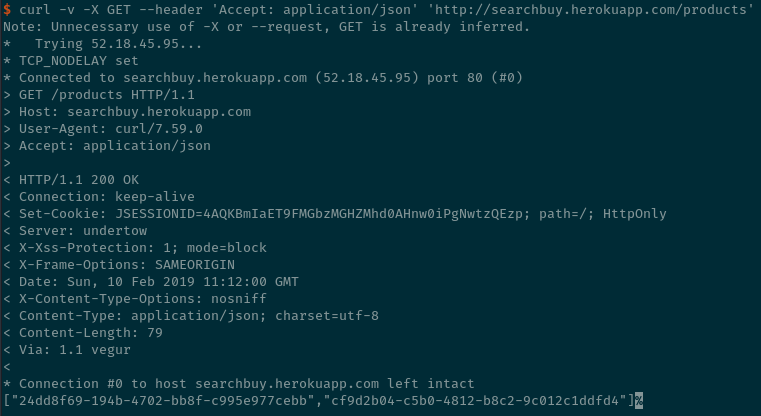
\includegraphics[width=.9\linewidth]{img/products-screen/get-products.png}
\end{center}
\subsubsection{POST \texttt{/products}}
\label{sec:org82cb4a6}
Aggiunge un prodotto
\begin{center}
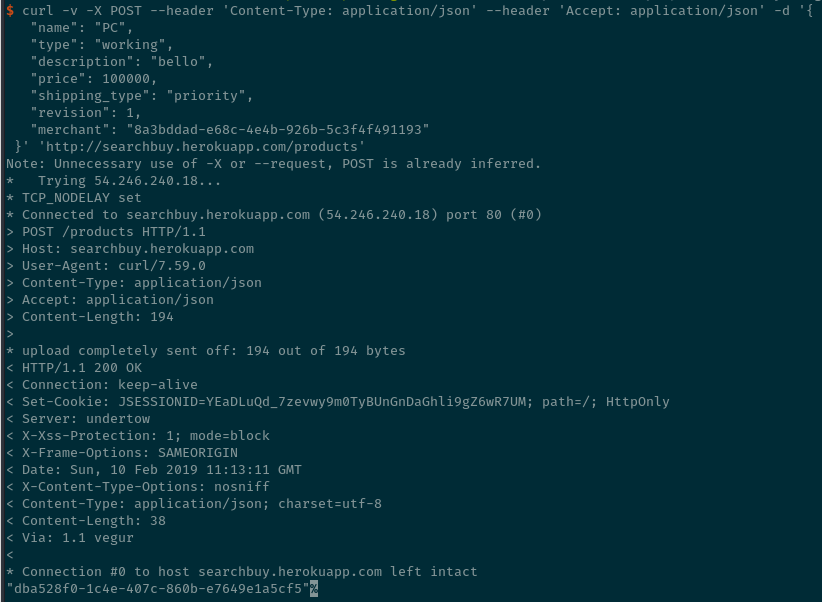
\includegraphics[width=.9\linewidth]{img/products-screen/post-products.png}
\end{center}
\subsubsection{GET \texttt{/products/:id}}
\label{sec:org223c125}
Restituisce tutte le informazioni riguardate un prodotto
\begin{center}
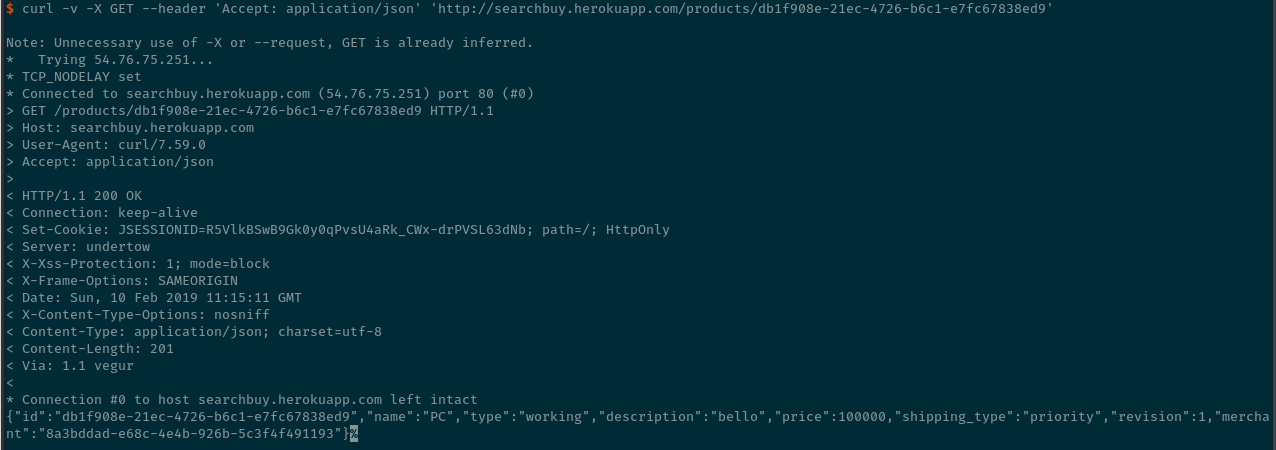
\includegraphics[width=.9\linewidth]{img/products-screen/get-product.png}
\end{center}
\subsubsection{PUT \texttt{/products/:id}}
\label{sec:org20c6544}
Modifica le informazioni riguardanti in prodotto
\begin{center}
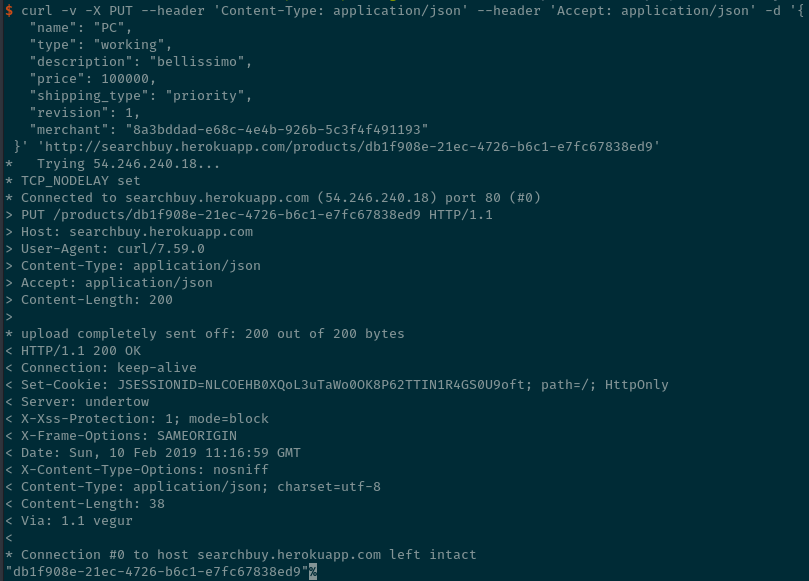
\includegraphics[width=.9\linewidth]{img/products-screen/put-product.png}
\end{center}
\subsubsection{DELETE \texttt{/products/:id}}
\label{sec:org871b24f}
Elimina un prodotto
\begin{center}
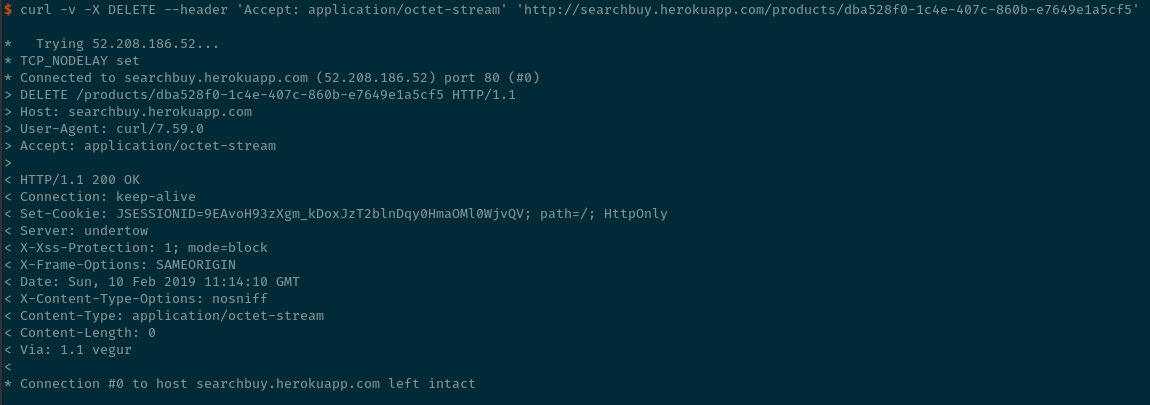
\includegraphics[width=.9\linewidth]{img/products-screen/delete-product.png}
\end{center}

\subsection{Venditori}
\label{sec:org77c0a9e}
\subsubsection{GET \texttt{/merchants}}
\label{sec:org7b12301}
Restituisce gli id dei venditori
É possibile fare una ricerca per nome passando il parametro \texttt{q} e il nome da cercare o le prime lettere del nome
\begin{center}
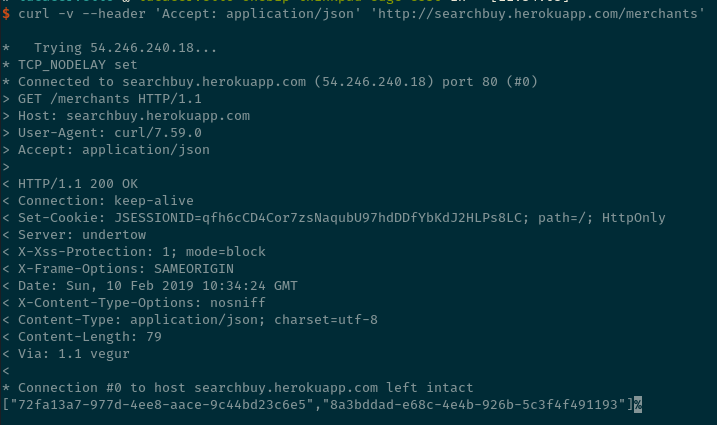
\includegraphics[width=.9\linewidth]{img/merchants-screen/get-merchants.png}
\end{center}
\subsubsection{POST \texttt{/merchants}}
\label{sec:orgd6c9cbd}
Aggiunge un venditore
\begin{center}
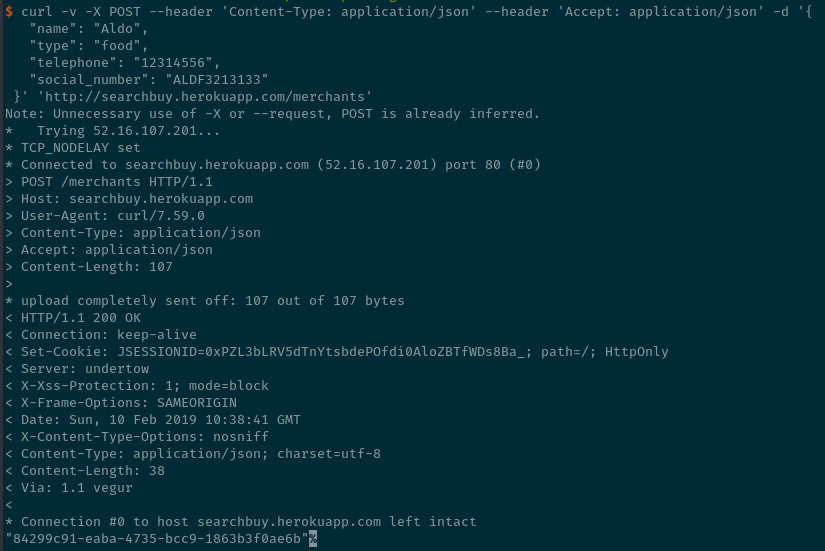
\includegraphics[width=.9\linewidth]{img/merchants-screen/post-merchants.png}
\end{center}
\subsubsection{GET \texttt{/merchants/:id}}
\label{sec:org6e45e42}
Restituisce tutte le informazioni riguardate un venditore
\begin{center}
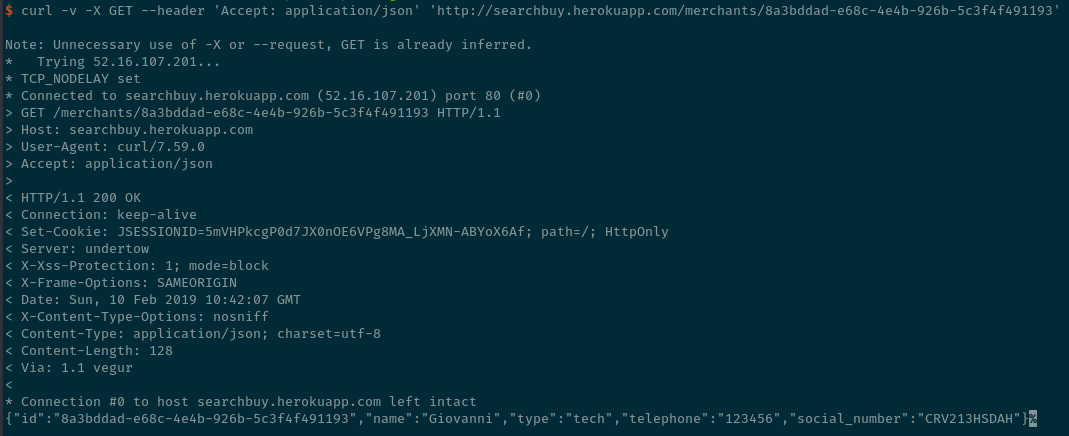
\includegraphics[width=.9\linewidth]{img/merchants-screen/get-merchant.png}
\end{center}
\subsubsection{PUT \texttt{/merchants/:id}}
\label{sec:org7caf974}
Modifica le informazioni riguardanti in venditore
\begin{center}
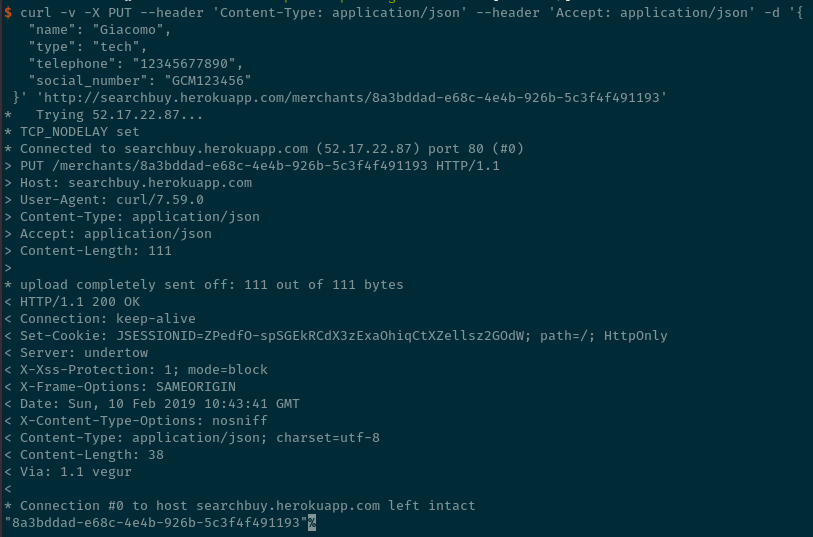
\includegraphics[width=.9\linewidth]{img/merchants-screen/put-merchant.png}
\end{center}
\subsubsection{DELETE \texttt{/merchants/:id}}
\label{sec:orgcba788f}
Elimina un venditore
\begin{center}
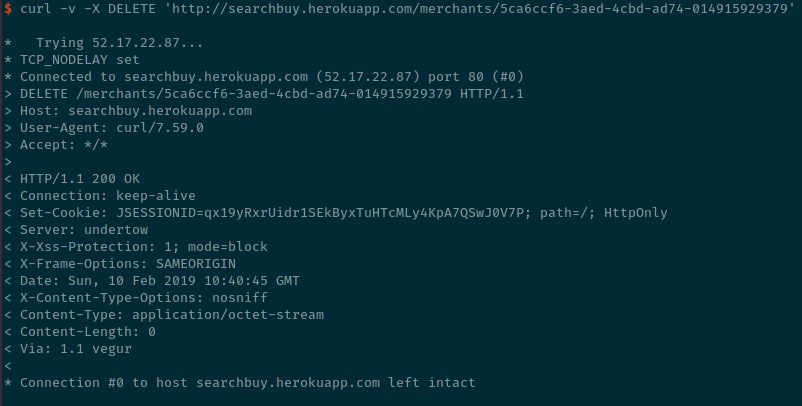
\includegraphics[width=.9\linewidth]{img/merchants-screen/delete-merchant.png}
\end{center}
\subsubsection{GET \texttt{/merchants/:id/products}}
\label{sec:org63157a0}
Restituisce gli id di tutti i prodotti del venditore
\begin{center}
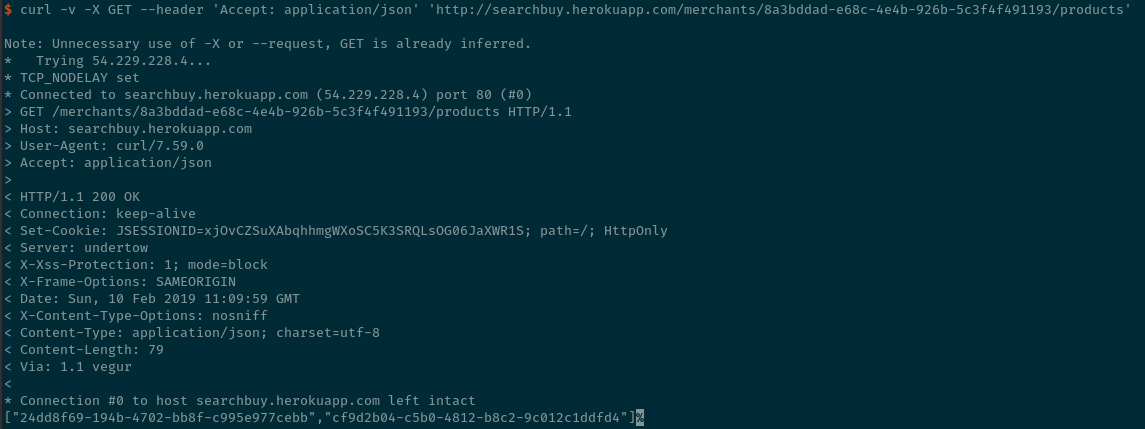
\includegraphics[width=.9\linewidth]{img/merchants-screen/get-products-merchants.png}
\end{center}
\subsection{Utenti}
\label{sec:org728556a}
\subsubsection{GET \texttt{/users}}
\label{sec:org1990a08}
Restituisce gli id dei utenti
É possibile fare una ricerca per nome passando il parametro \texttt{q} e il nome da cercare o le prime lettere del nome
\begin{center}
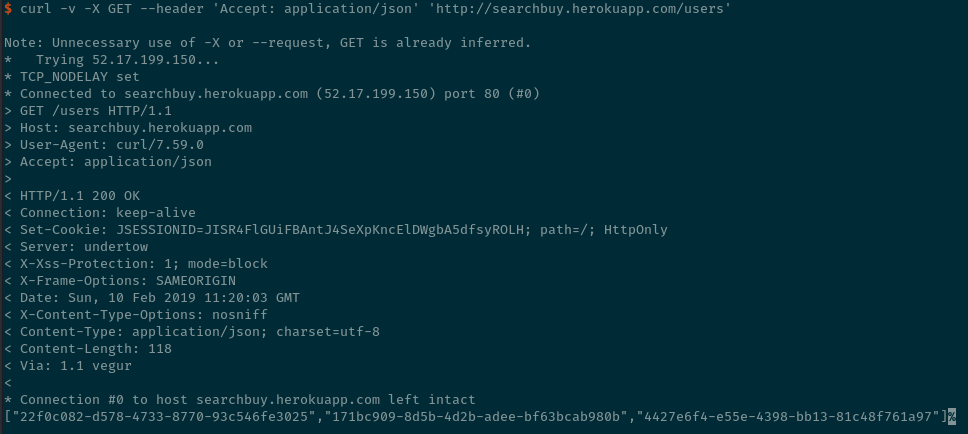
\includegraphics[width=.9\linewidth]{img/users-screen/get-users.png}
\end{center}
\subsubsection{POST \texttt{/users}}
\label{sec:org12f3c3d}
Aggiunge un utente
\begin{center}
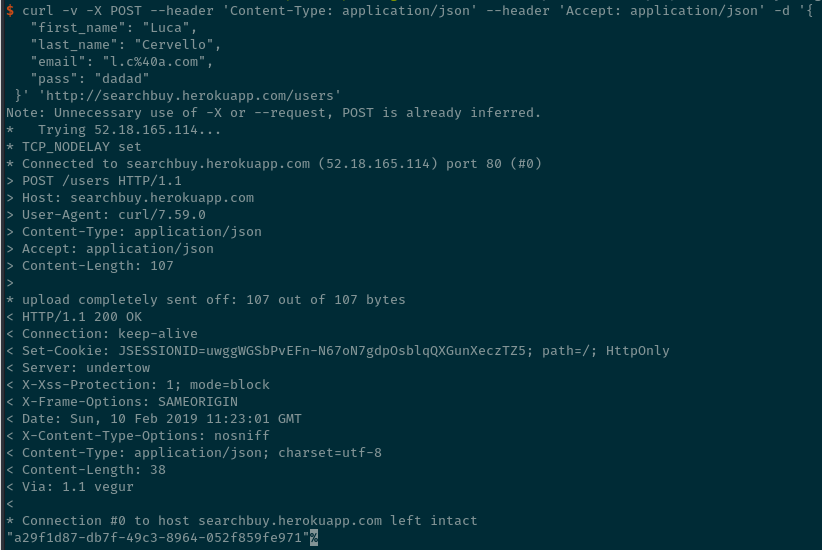
\includegraphics[width=.9\linewidth]{img/users-screen/post-users.png}
\end{center}
\subsubsection{GET \texttt{/users/:id}}
\label{sec:org88779f4}
Restituisce tutte le informazioni riguardate un utente
\begin{center}
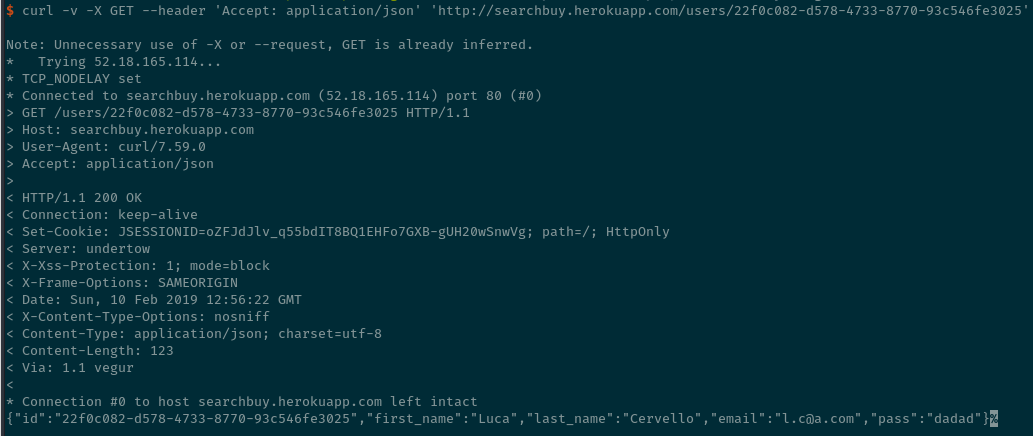
\includegraphics[width=.9\linewidth]{img/users-screen/get-user.png}
\end{center}
\subsubsection{PUT \texttt{/users/:id}}
\label{sec:org5ce5131}
Modifica le informazioni riguardanti in utente
\begin{center}
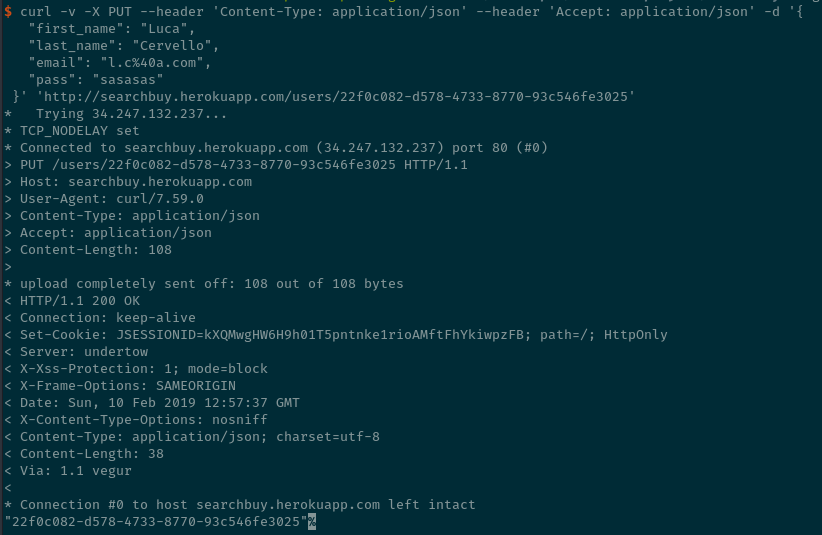
\includegraphics[width=.9\linewidth]{img/users-screen/put-user.png}
\end{center}
\subsubsection{DELETE \texttt{/users/:id}}
\label{sec:orgcf5f458}
Elimina un utente
\begin{center}
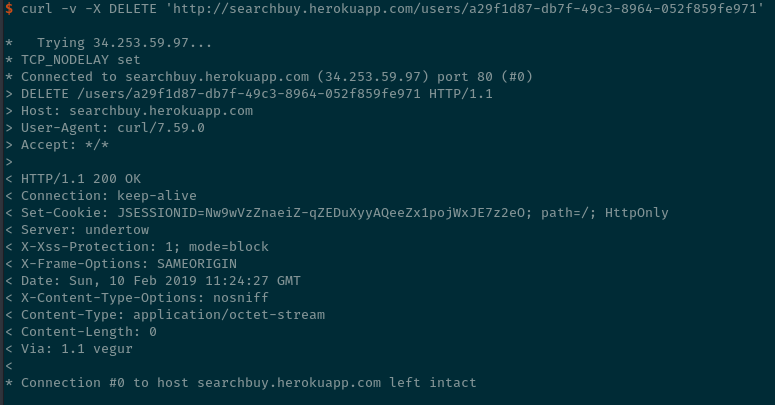
\includegraphics[width=.9\linewidth]{img/users-screen/delete-user.png}
\end{center}
\subsubsection{GET \texttt{/users/:id/preferences}}
\label{sec:org98626a4}
Restituisce tutte le informazioni riguardanti le preferenze
\begin{center}
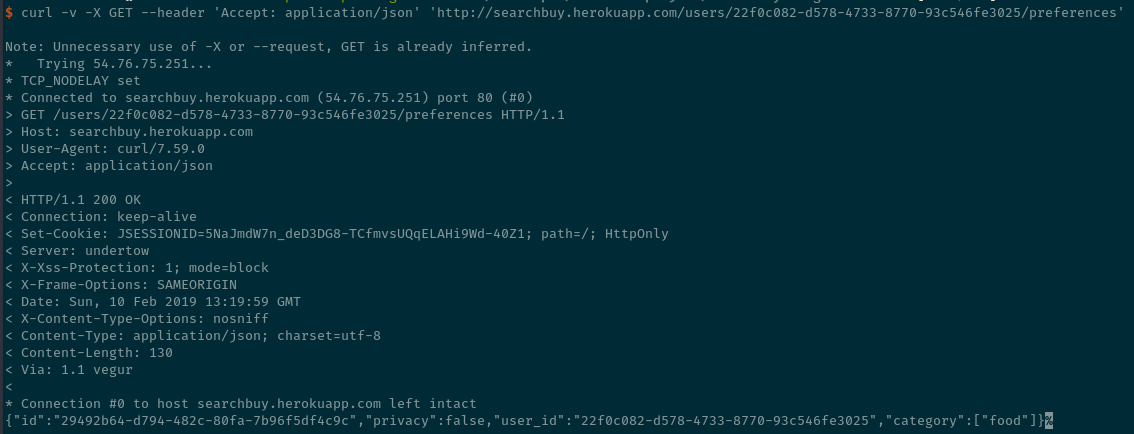
\includegraphics[width=.9\linewidth]{img/users-screen/get-preferences.png}
\end{center}
\subsubsection{POST \texttt{/users/:id/preferences}}
\label{sec:org0b4f868}
Aggiunge le preferenze per l'utente
\begin{center}
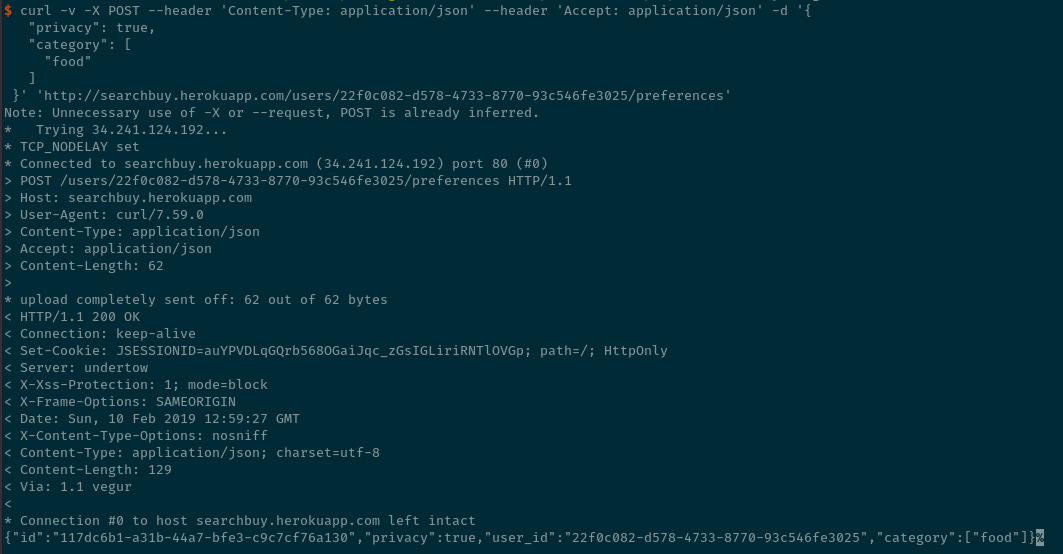
\includegraphics[width=.9\linewidth]{img/users-screen/post-preferences.png}
\end{center}
\subsubsection{PUT \texttt{/users/:id/preferences}}
\label{sec:org853f122}
Modifica le preferenze per l'utente
\begin{center}
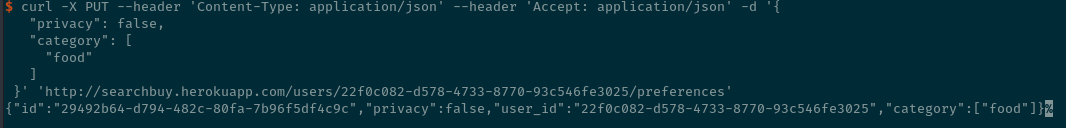
\includegraphics[width=.9\linewidth]{img/users-screen/put-preferences.png}
\end{center}
\subsubsection{DELETE \texttt{/users/:id/preferences}}
\label{sec:org44891e9}
Elimina le preferenze per l'utente
\begin{center}
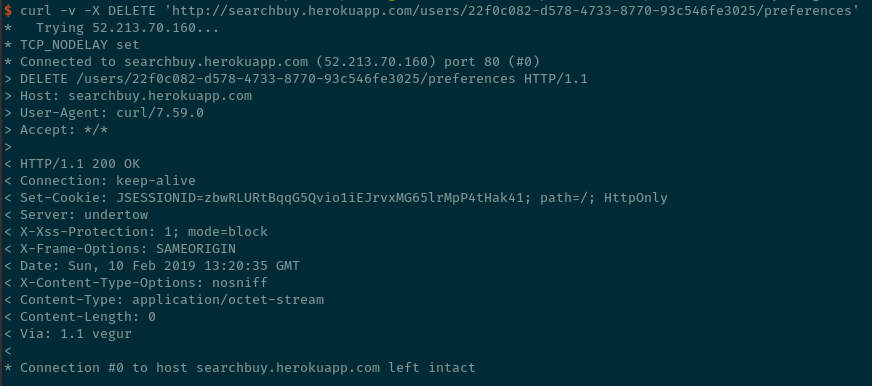
\includegraphics[width=.9\linewidth]{img/users-screen/delete-preferences.png}
\end{center}
\subsubsection{GET \texttt{/users/:id/orders}}
\label{sec:org9ac8ce3}
Restituisce tutti gli id degli ordini dell'utente
\begin{center}
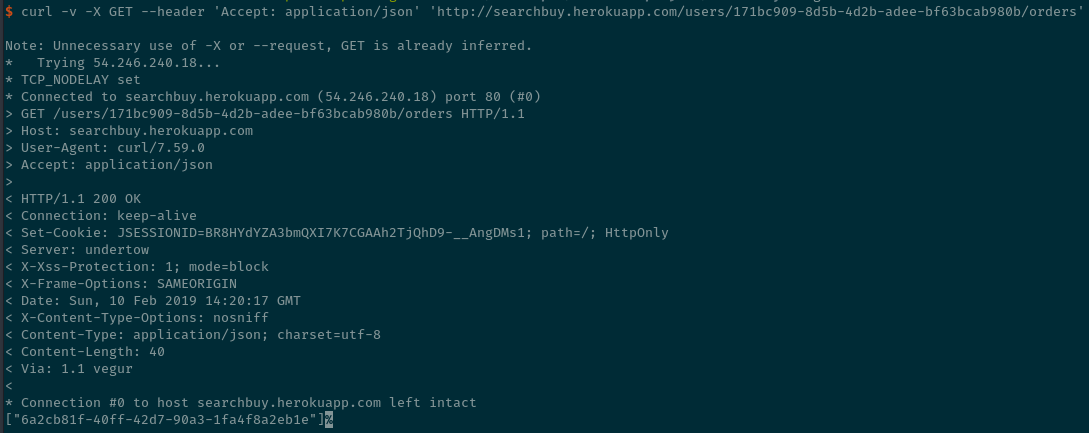
\includegraphics[width=.9\linewidth]{img/users-screen/get-user-orders.png}
\end{center}
\subsection{Ordini}
\label{sec:orga440d49}
\subsubsection{GET \texttt{/orders}}
\label{sec:orgd5d758a}
Restituisce tutti gli id degli ordini
\begin{center}
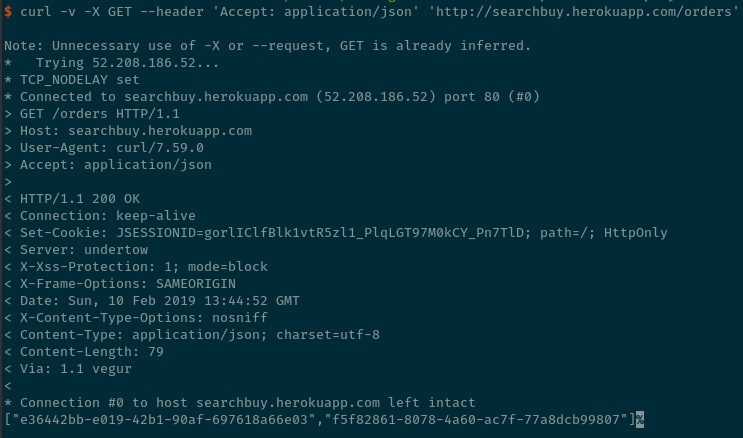
\includegraphics[width=.9\linewidth]{img/orders-screen/get-orders.png}
\end{center}
\subsubsection{POST \texttt{/orders}}
\label{sec:orga6950b2}
Aggiunge un ordine
\begin{center}
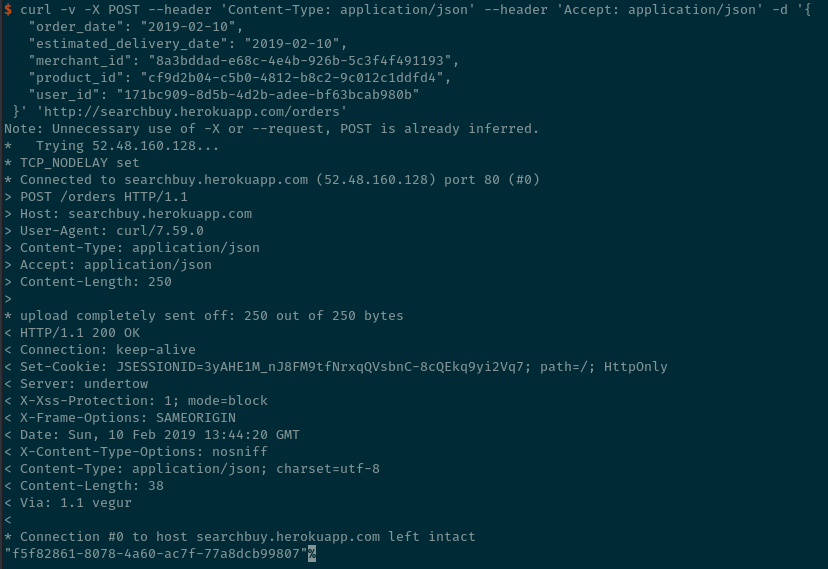
\includegraphics[width=.9\linewidth]{img/orders-screen/post-orders.png}
\end{center}
\subsubsection{GET \texttt{/orders/:id}}
\label{sec:org9bbc5ef}
Restituisce tutte le informazioni riguardate un ordine
\begin{center}
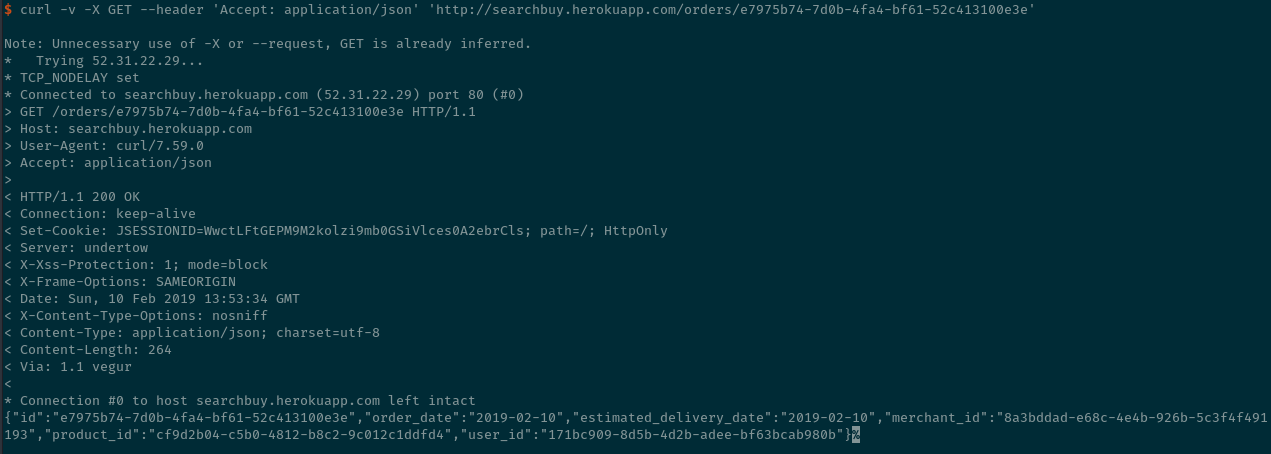
\includegraphics[width=.9\linewidth]{img/orders-screen/get-order.png}
\end{center}
\subsubsection{PUT \texttt{/orders/:id}}
\label{sec:orgf05adef}
Modifica le informazioni riguardanti in ordine
\begin{center}
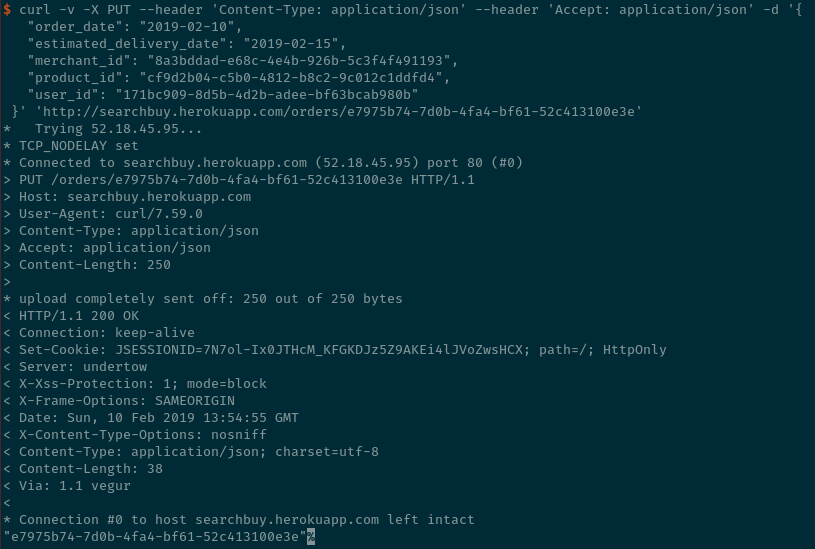
\includegraphics[width=.9\linewidth]{img/orders-screen/put-order.png}
\end{center}
\subsubsection{DELETE \texttt{/orders/:id}}
\label{sec:org08aba9f}
Elimina un ordine
\begin{center}
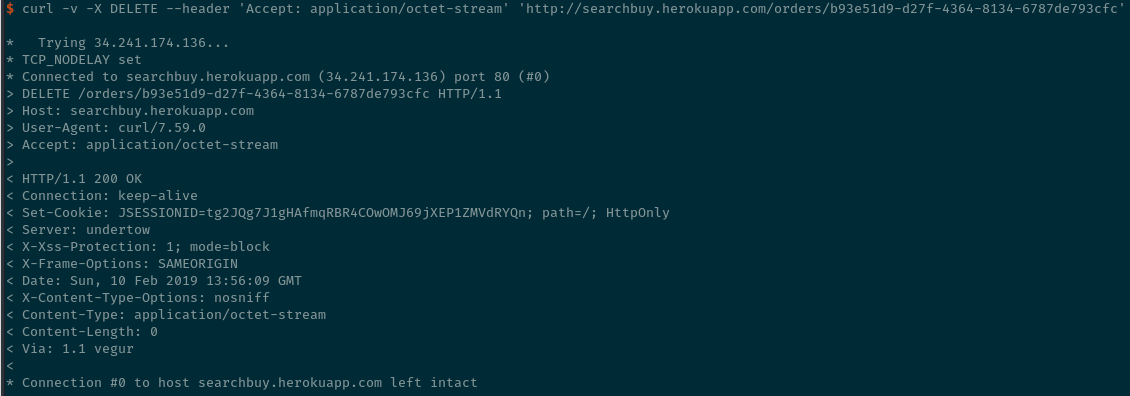
\includegraphics[width=.9\linewidth]{img/orders-screen/delete-order.png}
\end{center}
\end{document}
